\chapter{酸 碱 盐}

在前面几章里,我们已经学习过好多种化合物。自然界存在的和人工制造的化合物有几百万种之多,我们不可能一个个地进行学习。
人们经过长时间的实践,知道根据化合物的组成和性质来分成若干类,按类来学习和研究就比较简便。
本章要学习的酸、碱、盐,就是几类重要的化合物。

酸、碱、盐在日常生活中和在工农业生产上都有广泛的应用。
因此,学习酸、碱、盐的基础知识,不仅使我们能比较系统地学习化合物的组成、性质和相互关系,
而且可以了解酸、碱、盐在日常生活和社会主义建设中的重要意义。


\section{电解质和非电解质}\label{sec:5-1}

\subsection{溶液的导电性}

在上一章,我们已经学习了溶液的一些性质,现在我们来研究一下不同溶质的水溶液的导电性。

\begin{wrapfigure}[10]{r}{7cm}
    \centering
    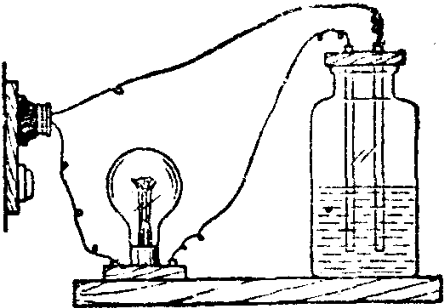
\includegraphics[width=5cm]{../pic/czhx1-ch5-1}
    \caption{试验物质的导电性}\label{fig:5-1}
\end{wrapfigure}

\wrapfiguretrick

\begin{shiyan}
    图 \ref{fig:5-1} 表示的是试验物质导电性的装置,其中主要包括盛有待试验物质的容器、石墨电极和显示电路里有无电流通过的电灯泡等三部分。

    在容器里依次分别加入干燥的食盐晶体、硝酸钾晶体、氢氧化钠晶体、无水硫酸、
    蒸馏水、食盐溶液、硝酸钾溶液、氢氧化钠溶液、硫酸溶液、酒精溶液和蔗糖溶液。
    连接直流电源以后,观察灯泡是不是发光。
\end{shiyan}


从上面的实验可以看到,干燥的食盐晶体、硝酸钾晶体、氢氧化钠晶体、无水硫酸都不导电,
蒸馏水也不导电\footnote{严格地说,蒸馏水也能导电,只是导电能力非常弱,用上述实验装置不能测出。},
可是,食盐、硝酸钾、氢氧化钠、硫酸的水溶液却能够导电。

食盐、硝酸钾和氢氧化钠,不但它们的水溶液能够导电,而且在熔化状态时也能够导电。
蔗糖和酒精就不同,它们的纯净物或水溶液都不能够导电。

\begin{shiyan}
    取几克硝酸钾晶体(或其它易熔的盐如氯化锌、氯化亚锡等)加入瓷坩埚内,放在三脚架和泥三角上,
    插入电极,加热到硝酸钾晶体熔化。连接直流电源,观察灯泡是不是发光。
\end{shiyan}

从上面的实验可以看到,熔化的硝酸钾能够导电。
凡是在水溶液里或熔化的状态下能够导电的化合物叫做\zhongdian{电解质},
在上述情况下都不能导电的化合物叫做\zhongdian{非电解质}。
例如,食盐、硝酸钾、氢氧化钠、硫酸等都是电解质,蔗糖、酒精等都是非电解质。


\subsection{电解质的电离}

为什么食盐、硝酸钾、氢氧化钠等物质在干燥时不导电,而溶于水或熔化时却能导电呢?
为了解决这个问题,必须对这些物质的结构和它们在熔化或溶解的条件下发生的变化进行分析。
我们知道,电流是由带电微粒按一定方向移动而形成的。
例如,金属能够导电,就是由于金属中存在能够自由移动的、带负电的电子。
电解质的水溶液(或熔化而成的液体)既然能够导电,那么,
在这些溶液(或熔化而成的液体)里,是不是也存在着能够自由移动的、带电的微粒呢?
如果有微粒存在,是哪种微粒呢?它们又是怎样形成的呢?下面我们以食盐为例来说明。

我们已经知道,在食盐的晶体里含有带正电的钠离子(\ce{Na+})和带负电的氯离子(\ce{Cl-}),
由于静电的作用,它们既互相吸引,又互相排斥,按一定规则紧密地排列着,
这些离子不能自由移动,因而干燥的食盐不能导电。
当食盐在水里溶解时,在水分子的作用下,减弱了钠离子和氯离子之间的吸引力,
使食盐晶体离解成能自由移动的带电的钠离子和氯离子(图 \ref{fig:5-2})\footnote{严格地说,是形成了与水结合着的钠离子和氯离子。}。
当食盐溶液中插入电极,连接直流电源时,带正电的钠离子向阴极移动,带负电的氯离子向阳极移动,因而食盐溶液就能够导电。

\begin{figure}[htbp]
    \centering
    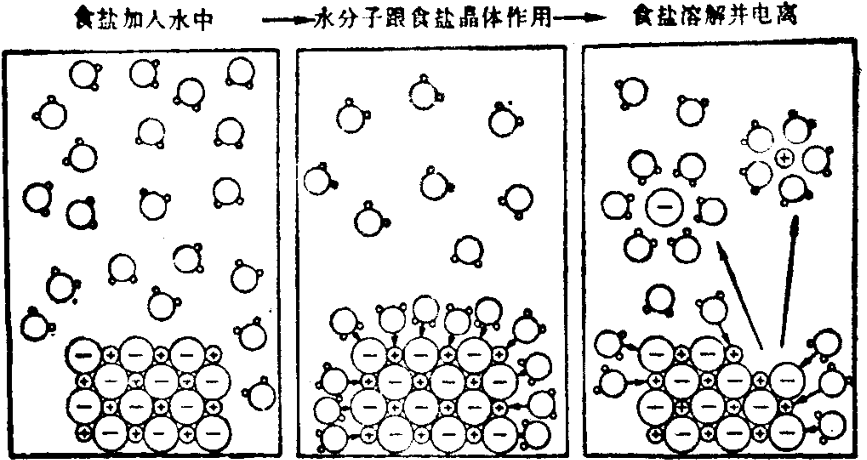
\includegraphics[width=12cm]{../pic/czhx1-ch5-2}
    \caption{食盐在水里的溶解和电离}\label{fig:5-2}
\end{figure}


食盐晶体受热熔化时,由于离子的运动随温度升高而加快,克服了带不同电荷的离子间的引力,
产生了能自由移动的钠离子和氯离子,因而食盐在熔化状态也能导电。

\zhongdian{电解质溶解于水或受热熔化时,离解成自由移动的离子的过程,叫做电离。}

电解质的电离可用如下的电离方程式来表示:
\begin{fangchengshi}
    \begin{aligned}
        & \ce{ \underset{\text{氯化钠}}{\ce{NaCl}} = Na+ + Cl- } \\
        & \ce{ \underset{\text{氢氧化钠}}{\ce{NaOH}} = Na+ + OH- } \\
        & \ce{ \underset{\text{硫酸}}{\ce{H2SO4}} = 2H+ + SO4^{2-} } \\
    \end{aligned}
\end{fangchengshi}

氢氧根离子(\ce{OH-})、硫酸根离子(\ce{SO4^{2-}})都是带电的原子团。
可见,离子不但是带正电或负电的原子,而且也可能是带正电或负电的原子团。

离子所带电荷一般可以根据它们在化合物中的化合价来判断。
例如,金属原子容易失去电子,化合价都是正的,金属离子都带正电,
它的化合价等于几,就可以判断,它带几个正电荷。

电解质溶液里,所有阳离子带的正电荷总数和所有阴离子带的负电荷总数是相等的,
所以整个溶液不显电性。


\begin{xiti}

\xiaoti{为什么用湿手接触正在通电的电器设备更容易发生触电事故?}

\xiaoti{金属能够导电,它们是不是电解质?食盐晶体不能导电,它是不是非电解质?为什么?}

\xiaoti{有人说:“电解质通过电流的时候发生电离”,这句话对吗?为什么?}

\xiaoti{硫酸铜、硝酸钾、硫酸钠、氢氧化钙都是电解质,写出它们在水溶液里的电离方程式。}

\end{xiti}


\section{酸、碱、盐是电解质}\label{sec:5-2}

我们已经知道,根据化合物在溶液里或熔化状态的导电性,它们可以分为电解质和非电解质两大类。
现在我们来学习几类重要的电解质。

\subsection{酸}

\begin{shiyan}
    用图 \ref{fig:5-1} 中所示的实验装置,分别试验盐酸和硝酸溶液的导电性。
\end{shiyan}

实验表明,盐酸和硝酸溶液都能够导电,它们跟硫酸一样,都是电解质。它们的电离方程式如下:
\begin{fangchengshi}
    \ce{ \underset{\text{盐酸}}{\ce{HCl}} = H+ + Cl- } \\
    \ce{ \underset{\text{硝酸}}{\ce{HNO3}} = H+ + NO3- } \\
    \ce{ \underset{\text{硫酸}}{\ce{H2SO4}} = 2H+ + SO4^{2-} }
\end{fangchengshi}

由上式可以看出,盐酸、硝酸、硫酸在水溶液里都能电离生成氢离子(\ce{H+})。

\zhongdian{电解质电离时所生成的阳离子全部是氢离子的化合物叫做酸。}
盐酸、硝酸和硫酸都属于酸类。

在酸的分子里,除去在水溶液里能够电离生成的氢离子,余下的部分是酸根离子,
例如,\ce{Cl-}、\ce{NO3-}、\ce{SO4^{2-}} 都是酸根离子。
酸根离子所带负电荷的数目等于酸分子电离时生成的氢离子的数目。


\subsection{碱}

\begin{shiyan}
    用图 \ref{fig:5-1} 中所示的装置,分别试验氢氧化钾和氢氧化钡的溶液的导电性。
\end{shiyan}

实验表明,氢氧化钾和氢氧化钡的溶液都能够导电,它们跟氢氧化钠一样,都是电解质。它们的电离方程式如下:
\begin{fangchengshi}
    \ce{ \underset{\text{氢氧化钾}}{\ce{KOH}} = K+ + OH- } \\
    \ce{ \underset{\text{氢氧化钡}}{\ce{Ba(OH)2}} = Ba^{2+} + 2OH- } \\
    \ce{ \underset{\text{氢氧化钠}}{\ce{NaOH}} = Na+ + OH- }
\end{fangchengshi}

由上式可以看出,氢氧化钾、氢氧化钡和氢氧化钠在水溶液里都能电离生成能自由移动的氢氧根离子(\ce{OH-})。

\zhongdian{电解质电离时所生成的阴离子全部是氢氧根离子的化合物叫做碱。}
氢氧化钠、氢氧化钾、氢氧化钡都属于碱类。

由以上所举各例可知,碱在电离的时候,除生成氢氧根离子外,还生成金属离子。
氢氧根离子带一个负电荷,因此,在碱里跟一个金属离子结合的氢氧根离子的数目等于这种金属离子所带正电荷的数目。


\subsection{盐}

\begin{shiyan}
    用图 \ref{fig:5-1} 所示的分别试验碳酸钠、硫酸镁、氯化钡等物质的溶液的导电性。
\end{shiyan}

实验表明,碳酸钠、硫酸镁、氯化钡等物质的溶液都能够导电,它们跟氯化钠一样,都是电解质。它们的电离方程式如下:
\begin{fangchengshi}
    \ce{ \underset{\text{碳酸钠}}{\ce{Na2CO3}} = 2Na+ + CO3^{2-} } \\
    \ce{ \underset{\text{硫酸镁}}{\ce{MgSO4}} = Mg^{2+} + SO4^{2-} } \\
    \ce{ \underset{\text{氯化钡}}{\ce{BaCl2}} = Ba^{2+} + 2Cl- } \\
    \ce{ \underset{\text{氯化钠}}{\ce{NaCl}} = Na+ + Cl- }
\end{fangchengshi}

由上列各式可以看出,碳酸钠、硫酸镁、氯化钡、氯化钠等物质在水溶液里都能电离出金属离子和酸根离子。
象这种\zhongdian{由金属离子和酸根离子组成的化合物叫做盐。}
其中金属离子所带正电荷的总数等于酸根离子所带负电荷的总数。


\begin{xiti}

\xiaoti{写出下列酸的电离方程式:\\
    \ce{HBr}, \quad  \ce{HClO3}, \quad \ce{HI}。
}


\xiaoti{写出下列碱的电离方程式:\\
    \ce{LiOH}, \quad \ce{Ca(OH)2}, \quad \ce{Ba(OH)2}。
}

\xiaoti{写出下列盐的电离方程式:\\
    \ce{FeCl3}, \quad \ce{CuSO4}, \quad  \ce{Ca(NO3)2}, \quad \ce{Al2(SO4)3}。
}

\xiaoti{硫酸氢钠(\ce{NaHSO4}) 溶于水时有 \ce{H+} 生成,它是不是一种酸?为什么?}

\end{xiti}


\section{常见的酸}\label{sec:5-3}

我们已经知道,酸是一类电解质,它们在电离时生成的阳离子全部是氢离子。
我们已经知道的硫酸、盐酸、碳酸、醋酸都属于酸。现在我们来学习几种常见的、重要的酸。


\subsection{盐酸(\ce{HCl})}

盐酸是氯化氢气体的水溶液。

\begin{shiyan}
    观察纯净的浓盐酸和工业品浓盐酸的颜色、状态以及它们在空气里形成的白雾。
    用手轻轻地在瓶口扇动,小心地闻盐酸的气味。
\end{shiyan}

纯净的浓盐酸是没有颜色的液体,有刺激性气味。
工业品的浓盐酸常因含有杂质而带黄色。
常用的浓盐酸约含 $37\%$ 的氯化氢,密度是 $1.19 \; \kmlflm$。
浓盐酸在空气里会生成白雾,这是因为从浓盐酸挥发出来的氯化氢气体跟空气里的水蒸气接触,
形成盐酸小液滴的缘故。盐酸有酸味,有腐蚀性。

\begin{shiyan}
    把紫色石蕊试液和无色酚酞试液分别加入两个盛有稀盐酸的试管里,观察溶液的颜色有什么变化。
\end{shiyan}

\begin{shiyan}
    把紫色石蕊试液和无色酚酞试液分别加入两个盛有氢氧化钠稀溶液的试管里,观察溶液颜色有什么变化。
\end{shiyan}

石蕊试液遇盐酸变成红色,酚酞试液遇盐酸不变色。
石蕊试液遇碱溶液变蓝色,酚酞试液碱溶滚变红色。
象石蕊和酚酞这能跟酸或碱的溶液起作用而显示不同颜色的物质,叫做\zhongdian{酸碱指示剂},
通常也简称\zhongdian{指示剂}。

盐酸还能跟多种金属、金属氧化物、金属氢氧化物等物质起反应,下面简单介绍盐酸的其它化学性质。


\subsubsection{盐酸跟金属的反应}

\begin{shiyan}
    把锌粒和铁屑分别放入盛有稀盐酸的两个试管里,观察发生的变化。试验产生的气体是不是氢气。
\end{shiyan}

盐酸跟锌、铁起置换反应,分别生成氢气、氯化锌或氯化亚铁。
\begin{fangchengshi}
    \ce{ Zn + 2HCl = \underset{\text{氯化锌}}{\ce{ZnCl2}} + H2 ^ } \\
    \ce{ Fe + 2HCl = \underset{\text{氯化亚铁}}{\ce{FeCl2}} + H2 ^ }
\end{fangchengshi}


\subsubsection{盐酸跟金属氧化物的反应}

\begin{shiyan}
    把一根生锈的铁钉放入盛有稀盐酸的试管里,过一会儿取出,用水洗净,观察铁钉表面的变化。
\end{shiyan}

从实验看出,铁钉表面的锈已被除去,这是因为盐酸跟铁锈(主要成分是 \ce{Fe2O3 . H2O} ) 起反应,
生成可溶性的氯化铁的缘故。
\begin{fangchengshi}
    \ce{ Fe2O3 + 6HCl = \underset{\text{氯化铁}}{\ce{2FeCl3}} + 3H2O }
\end{fangchengshi}

由于盐酸跟金属氧化物起反应后生成可溶性物质,金属制品在电镀、焊接等操作前可以用盐酸来清除表面上的锈。


\subsubsection{盐酸跟碱的反应}

\begin{shiyan}
    在盛有少量氢氧化铜的试管里,加入适量的盐酸,观察发生的变化。
\end{shiyan}

从实验看出,盐酸跟不溶于水的氢氧化铜起反应,生成能溶于水的氯化铜。
\begin{fangchengshi}
    \ce{ Cu(OH)2 + 2HCl = \underset{\text{氯化铜}}{\ce{CuCl2}} + 2H2O }
\end{fangchengshi}



\subsubsection{盐酸跟硝酸银的反应}

\begin{shiyan}
    在盛有少量稀盐酸的试管里,滴入几滴硝酸银溶液和几滴稀硝酸\footnote{加入几滴稀硝酸是为了防止某些杂质的干扰。},观察发生的现象。
\end{shiyan}

从实验看出,盐酸跟硝酸银起反应,生成不溶于硝酸的氯化银凝乳状白色沉淀。
\begin{fangchengshi}
    \ce{ HCl + \underset{\text{硝酸银}}{\ce{AgNO3}} = \underset{\text{氯化银}}{\ce{AgCl}} v + HNO3 }
\end{fangchengshi}

这个反应可以用于检验盐酸,也可用于检验氯化钠等可溶性氯化物,因为反应后都生成不溶于硝酸的氯化银。
\begin{fangchengshi}
    \ce{ NaCl + AgNO3 = AgCl v + NaNO3 }
\end{fangchengshi}

在以上两个反应里,参加反应的两种化合物互相交换成分,生成另外两种化合物。
象这类\zhongdian{由两种化合物互相交换成分,生成另外两种化合物的反应,叫做复分解反应。}

盐酸是一种重要的化工产品。除用于金属表面的除锈外,还用于制造氯化锌等氯化物,
以及某些药剂和试剂。人的胃液里含有少量的盐酸,可以帮助消化。



\subsection{硫酸(\ce{H2SO4})}

\begin{shiyan}
    观察浓硫酸的颜色和状态。用玻璃棒蘸浓硫酸在纸上写字,过一会儿,观察纸上有什么变化。
    用火柴梗蘸一点浓硫酸,放置一会儿,观察火柴梗有什么变化。
\end{shiyan}

纯净的浓硫酸是没有颜色、粘稠、油状的液体,不容易挥发。
常用浓硫酸的浓度是 $98\%$,密度是 $1.84 \; \kmlflm$。

浓硫酸有吸水性,跟空气接触,能够吸收空气里的水分,所以,它常用作某些气体的干燥剂。
浓硫酸也能够夺取纸张、木材、衣服、皮肤(它们都是由含碳、氢、氧等元素的化合物组成的)里的
水分\footnote{严格地说,浓硫酸能将这些物质中的氢、氧元素按水的组成比脱去,这种作用通常叫做脱水作用。},
使它们碳化。上面的实验里,纸和火柴梗的颜色变黑也就是发生了碳化的缘故。
硫酸对皮肤或衣服有很大的腐蚀性,如果不慎在皮肤或衣服上沾上硫酸,应立即用布拭去,再用水冲洗。

浓硫酸很容易溶解于水,同时放出大量的热。如果把水倒进浓硫酸里,水的比重较小,浮在硫酸上面,
溶解时放出的热会使水立刻沸腾,使硫酸液滴向四周飞溅。为了防止发生事故,
\zhongdian{稀释浓硫酸时,一定要把浓硫酸沿着器壁慢慢地注入水里,并不断搅动,
使产生的热量迅速地扩散。切不可把水倒进浓硫酸里。}


\begin{shiyan}
    把浓硫酸沿着烧杯壁缓慢地注入盛有水的烧杯里,用玻璃棒不断搅动,用手接触烧杯外壁,注意溶液温度有什么变化。
\end{shiyan}

稀硫酸也可使紫色的石蕊试液变红,无色的酚酞试液遇稀硫酸不变色。现将稀硫酸的其它化学性质简单介绍于下:

\subsubsection{稀硫酸跟金属的反应}

\begin{shiyan}
    在盛有稀硫酸的试管里,轻轻放入锌粒,观察发生的现象。
\end{shiyan}

稀硫酸跟锌起反应放出氢气,同时生成能溶于水的硫酸锌。
\begin{fangchengshi}
    \ce{ Zn + H2SO4 = ZnSO4 + H2 ^ }
\end{fangchengshi}


\subsubsection{稀硫酸跟金属氧化物的反应}

\begin{shiyan}
    在盛有稀硫酸的试管里,加入一个生锈的铁钉,稍加热,观察发生的变化。
\end{shiyan}

可以看到,铁钉上的锈逐渐消失。
\begin{fangchengshi}
    \ce{ Fe2O3 + 3H2SO4 = \underset{\text{硫酸铁}}{\ce{Fe2(SO4)3}} + 3H2O }
\end{fangchengshi}


\subsubsection{稀硫酸跟碱的反应}

\begin{shiyan}
    在盛有少量氢氧化铜的试管里,加入少量稀硫酸,现察发生的变化。
\end{shiyan}

可以看到,稀硫酸跟不溶于水的氢氧化铜起反应,生成能溶于水的硫酸铜。
\begin{fangchengshi}
    \ce{ Cu(OH)2 + H2SO4 = CuSO4 + 2H2O }
\end{fangchengshi}


\subsubsection{稀硫酸跟氯化钡的反应}

\begin{shiyan}
    在盛有少量稀硫酸的试管里,注入几滴氯化钡溶液和几滴稀硝酸\footnote{加入几滴稀硝酸是为了防止某些杂质的干扰。}, 观察发生的现象。
\end{shiyan}

从实验看出,稀硫酸跟氯化钡起反应,生成不溶于硝酸的白色硫酸钡沉淀。
\begin{fangchengshi}
    \ce{ H2SO4 + \underset{\text{氯化钡}}{\ce{BaCl2}} = \underset{\text{硫酸钡}}{\ce{BaSO4}} v + 2HCl }
\end{fangchengshi}

这个反应可用于检验硫酸,也可用于检验硫酸钠等可溶性的含硫酸根的盐,因为反应都生成不溶于硝酸的硫酸钡。
\begin{fangchengshi}
    \ce{ Na2SO4 + BaCl2 = BaSO4 v + 2NaCl }
\end{fangchengshi}

硫酸是一种非常重要的化工原料,广泛应用于生产化肥、农药、火药、染料以及冶炼有色金属、精炼石油、金属去锈等方面。



\subsection{硝酸(\ce{HNO3})}

\begin{shiyan}
    观察硝酸的状态和顔色。观察稀硝酸对石蕊试液和酚酞试液的颜色变化。
\end{shiyan}

纯净的硝酸是一种无色的液体,具有刺激性的气味。跟盐酸相似,在空气里也能挥发出 \ce{HNO3} 气体,
跟空气里的水蒸气结合成硝酸小液滴,形成白雾。
硝酸也能强烈地腐蚀皮肤和衣服,使用硝酸的时候,要特别小心。
硝酸溶液也能使紫色的石蕊试液变成红色,无色的酚酞试液遇硝酸溶液不变色。

硝酸的氧化性很强,它跟金属起反应的时候,一般生成水而不生成氢气。

硝酸也能跟金属氧化物象氧化锌、氧化镁等以及碱类象氢氧化锌、氢氧化镁等起反应,生成水和硝酸锌、硝酸镁等化合物。

硝酸是一种重要的化工原料,广泛应用于生产化肥、染料、火药等方面。

除上述三种酸以外,磷酸(\ce{H3PO4})也是一种常见的重要的酸。
磷酸是一种无色的晶体,容易吸收水分,易溶于水。
通常用的磷酸是一种糖浆状的水溶液,含有 $70—80\%$ 的磷酸。

磷酸对石蕊或酚酞试液的作用以及跟某些金属、金属氧化物、碱所起的反应都同盐酸、硫酸等相似。

磷酸的主要用途是制造磷肥。


\begin{xiti}

\xiaoti{对于化合、分解、置换、复分解等四种反应类型,各举出两个例子,写出它们的化学方程式。}

\xiaoti{1 克的锌和 1 克的铁分别跟足量的稀盐酸起反应,各生成多少克氢气?它们的体积各是多少升(在标准状况下)?}

\xiaoti{150 毫升密度为 $1.028 \; \kmlflm$ 的盐酸($6\%$ \ce{HCl})跟足量的硝酸银溶液起反应,计算生成的氯化银的质量。}

\xiaoti{在两个烧杯里分别盛 50 克浓硫酸和 50 克浓盐酸。在空气中放置一定时间后,二者的质量有什么变化?为什么?}

\xiaoti{现有浓度为 $98\%$,密度为 $1.84 \; \kmlflm$ 的浓硫酸,要配制 500 克 $20\%$ 硫酸,需用浓硫酸和水各多少毫升?怎样操作?}

\xiaoti{写出下列物质间反应的化学方程式:}
\begin{xiaoxiaotis}

    \xxt{铝跟硫酸,}
    \xxt{硝酸跟氢氧化钙,}
    \xxt{氧化铜跟硫酸。}

\end{xiaoxiaotis}


\xiaoti{有一块已部分氧化的锌片 42 克,跟足量稀硫酸反应完全后,生成氢气 $1.2$ 克,求锌片中锌的百分含量。}

\xiaoti{取 2 克含有杂质氯化钠的硫酸钠,溶于水后,滴加氯化钡溶液到沉淀不再生成为止,生成 $3.2$ 克硫酸钡,求硫酸钠含杂质的百分比。}

\end{xiti}


\section{酸的通性 pH值}\label{sec:5-4}

就人类认识事物的过程来说,总是由认识个别的和特殊的事物,逐步地扩大到认识一般的事物。
我们在学习了几种个别的酸的性质以后,就要逐步地扩大到认识酸的一般性质。

\subsection{酸的分类和命名}

根据酸的分子里是不是含有氧原子,可以把酸分成含氧酸和无氧酸两类。
硫酸、硝酸、磷酸、碳酸等是含氧酸,盐酸、氢硫酸(\ce{H2S})等是无氧酸。

根据酸分子电离时所能生成的氢离子的个数,可以把酸分成一元酸、二元酸、三元酸等。
例如,盐酸是一元酸,硫酸是二元酸,磷酸是三元酸。

含氧酸一般是根据它的分子里氢氧两元素以外的另一种元素的名称而命名为 “某酸”。
例如,\ce{H2SO4} 叫硫酸, \ce{HClO3} 叫氯酸, \ce{H3PO4} 叫磷酸等等。
无氧酸的命名,是在氢字的后面加上另一元素的名称,叫做 “氢某酸” 。
例如,\ce{HCl} 叫做氢氯酸(俗名盐酸), \ce{H2S} 叫做氢硫酸,等等。


\subsection{酸的通性}

由于酸在水溶液里都能电离,生成氢离子,所以,它们有一些相似的化学性质。

1. 酸溶液能跟酸碱指示剂起反应。例如,紫色的石蕊试液遇酸变红色,无色的酚酞试液遇酸不变色。

2. 酸能跟多种活泼金属起反应,通常生盐和氢气。

我们已经知道,锌和铁能分别跟盐酸起置换反应,生成氢气和相应的盐。
\begin{fangchengshi}
    \ce{ Zn + 2HCl = ZnCl2 + H2 ^ } \\[-0.5em]
    \ce{ Fe + 2Hcl = FeCl2 + H2 ^ }
\end{fangchengshi}

在这两个反应里,每个锌和铁的原子失去两个电子,它们的化合价都由 $0$ 价上升为 $+2$ 价,
每个氢原子接受一个电子,化合价由 $+1$ 价下降为 $0$ 价。这两个反应都属于氧化-还原反应。

是不是各种金属都能跟酸起置换反应呢?

\begin{shiyan}
    把铜和银各一小片分别放入盛有稀盐酸的两个试管里,观察有没有反应发生。
\end{shiyan}

由实验看出,铜和银跟稀盐酸不起反应,可见,金属跟酸反应与金属的性质有关。
经过长期的实践,人们总结出常见金属的化学活动性顺序如下:
\begin{center}
    \begin{tblr}{columns={c}}
        \ce{K} & \ce{Ca} & \ce{Na} & \ce{Mg} & \ce{Al} & \ce{Zn} & \ce{Fe}  & \ce{Sn} & \ce{Pb} & \ce{(H)} & \ce{Cu} &  \ce{Hg} & \ce{Ag} & \ce{Pt} & \ce{Au} \\
       \SetCell[c=15]{c} \tikz[overlay, >=Stealth] \draw [->] (-4, 0.5) -- (8.5, 0.5); 金属活动性由强逐渐减弱
    \end{tblr}
\end{center}
% \begin{center}
%     \begin{tblr}{columns={c}}
%         \ce{K}  \ce{Ca} \ce{Na} \ce{Mg} \ce{Al} \ce{Zn} \ce{Fe} \ce{Sn} \ce{Pb} \ce{(H)} \ce{Cu} \ce{Hg} \ce{Ag} \ce{Pt} \ce{Au} \\
%         \tikz[overlay, >=Stealth] \draw [->] (-2, 0.5) -- (6.5, 0.5); 金属活动性由强逐渐减弱
%     \end{tblr}
% \end{center}
% K Ca Na Mg Al Zn Fe Sn Pb (H) Cu Hg Ag Pt Au


\begin{wrapfigure}[23]{r}{4cm}
    \centering
    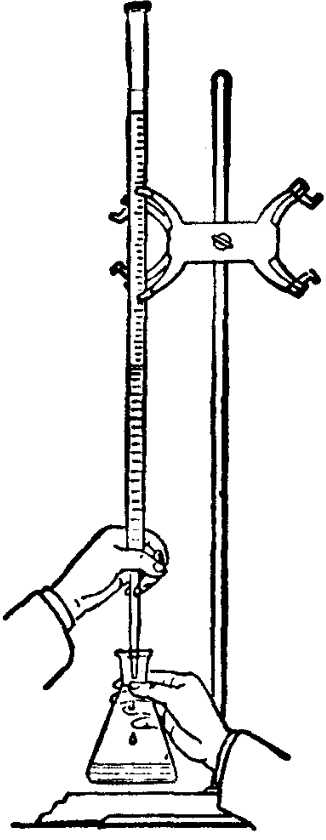
\includegraphics[width=3cm]{../pic/czhx1-ch5-3}
    \caption{\begin{minipage}[t]{2.5cm}
        用滴定管做\\
        中和反应实验
    \end{minipage}}\label{fig:5-3}
\end{wrapfigure}

在金属活动性顺序中,金属的位置越靠前,金属在水溶液中就越容易失去电子变成离子,它的活动性就越强。
在上列金属中,钾的活动性最强,钙次之,金的活动性最弱。排在氢前面的金属能置换出酸里的氢,
排在氢后面的金属不能置换出酸里的氢。

3. 酸能跟某些金属氧化物起反应,生成盐和水。例如:
\begin{fangchengshi}
    \ce{ CuO + H2SO4 = CuSO4 + H2O }
\end{fangchengshi}

4. 酸能跟某些盐起反应,生成另一种酸和另一种盐。例如:
\begin{fangchengshi}
    \ce{ AgNO3 + HCl = AgCl v + HNO3 }
\end{fangchengshi}


5. 酸跟碱起中和反应,生成盐和水。

\begin{shiyan}
    在盛有氢氧化钠溶液的锥形瓶里,滴入几滴酚酞试液,溶液变成红色。
    再用滴定管慢慢滴入稀盐酸,同时不断振荡溶液,一直到溶液刚刚变成无色为止(图 \ref{fig:5-3}) 。
\end{shiyan}

酚酞试液遇碱溶液变成红色,当滴入盐酸到酚酞试液刚刚变成无色时,溶液既不显酸性,也不显碱性。反应可用下式表示:
\begin{fangchengshi}
    \ce{ NaOH + HCl = NaCl + H2O }
\end{fangchengshi}

\zhongdian{酸跟碱作用而生成盐和水的反应,叫做中和反应。}

中和反应在工农业生产和科学实验中应用很广。例如,
在化工生产和科学实验里,当溶液里有过量酸或碱时,常用适量的碱或酸来中和;
在农业生产上,强酸性的土壤不适宜植物的生长,可以施入适量的熟石灰〔\ce{Ca(OH)2}〕来中和土壤里的酸,
就可以改良土壤,改善作物的生长条件。


\subsection{pH 值 —— 酸碱度的表示法}

在前边做过的实验里,我们曾用酸碱指示剂来试验溶液里是否含有酸或碱,也就是说,试验溶液是酸性还是碱性。
但是,在工农业生产和科学实验中,仅知道溶液是酸性还是碱性是不够的。还必须测定和控制溶液的酸碱性强弱程度,即溶液的酸碱度。

溶液的酸碱度常用 pH 值来表示,pH 值的范围通常在 0—14 之间(图 \ref{fig:5-4})。

\begin{figure}[htbp]
    \centering
    \begin{tikzpicture}[scale=0.8, >=Stealth,
    every node/.style={fill=white, inner sep=1pt},
]
    \draw (-0.5, 0) -- (14.5, 0);
    \foreach \x in {0, 1, ..., 14} {
        \ifnum \x = 7
            \draw (\x, -0.5) -- (\x, 0.4) node [above=0.1em] {$\x$};
        \else
            \draw (\x, 0) -- (\x, 0.2) node [above=0.2em] {$\x$};
        \fi
    }

    \draw [<->, very thick] (0.5, -1) -- (13.5, -1)
        node [midway] {中性}
        node [pos=0.2, below=0.5em] {酸性增强}
        node [pos=0.8, below=0.5em] {碱性增强};
\end{tikzpicture}


    \caption{pH 值和酸碱性}\label{fig:5-4}
\end{figure}

$\text{pH 值} = 7$ 时,溶液呈中性,\ce{H+} 离子和 \ce{OH-} 离子浓度相等。

$\text{pH 值} < 7$ 时,溶液呈酸性, pH 值越小,\ce{H+} 离子浓度越大,酸性越强。

$\text{pH 值} > 7$ 时,溶液呈碱性, pH 值越大,\ce{OH-} 离子浓度越大,碱性越强。

测定 pH 值的最简便的方法是使用 pH 试纸,这种试纸在不同酸碱度的溶液里,显示不同的颜色。
测定时,把待试溶液滴在 pH 试纸上,然后把试纸显示的颜色跟标准比色卡对照,便可知道溶液的 pH 值。
如果要精确地测定溶液的 pH 值,可以采用一种叫 pH 计的仪器。

\begin{shiyan}
    配制几种不同浓度的酸和碱的稀溶液,用 pH 试纸测定它们的 pH 值。
\end{shiyan}

\begin{shiyan}
    取 2 克土壤样品放在表面皿上,加蒸馏水 3 毫升,搅拌一分钟,静置澄清。用 pH 试纸测溶液的 pH 值。
\end{shiyan}

了解溶液的酸碱度,对工农业生产有重要的意义。例如,
在化工生产中,许多反应必须在一定酸碱度的溶液里才能进行。
在农业方面,土壤酸碱度的大小,对作物的生长也有很大的影响。
一般说来,大多数的作物适宜在中性或接近中性的土壤中生长。
当土壤的 pH 值小于 4 或大于 $8.5$ 时,一般作物难于生长。



\begin{xiti}

\xiaoti{把足量的稀硫酸加入盛有少量氧化铜和铜的混和物的试管里,加热后过滤,在滤纸上剩下什么物质?在滤液里有什么物质?}

\xiaoti{有两瓶溶液,一瓶溶液的 pH 值是 $4.5$, 另一瓶溶液的 pH 值是 $9.5$。在这两瓶溶液里,各滴入几滴酚酞试液,有什么现象发生?
    如果要使前一种溶液的 pH 值升高,后一种溶液的 pH 值降低,可以采取什么措施?
}

\xiaoti{某工厂化验室用 $15\%$ 的氢氧化钠溶液,洗涤一定量石油产品中的残余硫酸,共消耗这种溶液 40 克,
    洗涤后溶液呈中性,问在这一定量的石油产品里含硫酸多少克?
}

\xiaoti{把锌和铜的混和物 50 克和足量稀硫酸起反应,可制得氢气 $1.1$ 克,求这混和物里含锌和铜各多少克?}


\xiaoti{在家里用石灰水(碱性)、食醋(酸性)来试验一些植物色素,如红紫色的花瓣、果皮等,
    看它们的颜色发生什么变化。(如果用花瓣、果皮的汁液或酒精浸出液来试验,效果可以更好些。)
}

\end{xiti}


\section{常见的碱 碱的通性}\label{sec:5-5}

现在我们来学习两种常见的、重要的碱。

\subsection{氢氧化钠(\ce{NaOH})}

\begin{shiyan}
    用镊子取出一小块氢氧化钠放在表面皿上,观察它的状态、颜色,放置一会儿,再观察它的状态发生什么变化。
    把一小块氢氧化钠溶解在有少量水的试管里,注意溶液的温度有没有变化。
\end{shiyan}

纯净的氢氧化钠是一种白色固体,极易溶解于水,溶解时放出大量的热。它的水溶液有涩味和滑腻感。
暴露在空气里的氢氧化钠容易吸收水分而潮解。因此,氢氧化钠可用作某些气体的干燥剂。
由于氢氧化钠有强烈的腐蚀性,因此它又叫苛性钠、火碱或烧碱。
\zhongdian{在使用氢氧化钠时必须十分小心,防止皮肤、衣服被它腐蚀。}

下面简单介绍氢氧化钠的一些化学性质。

\subsubsection{氢氧化钠跟酸碱指示剂的反应}

氢氧化钠溶液能够使紫色的石蕊试液变成蓝色,使无色的酚酞试液变成红色。


\subsubsection{氢氧化钠跟非金属氧化物的反应}

氢氧化钠能跟二氧化碳、二氧化硫等非金属氧化物起反应。
\begin{fangchengshi}
    \ce{ 2NaOH + CO2 = \underset{\text{碳酸钠}}{\ce{Na2CO3}} + H2O } \\
    \ce{ 2NaOH + SO2 = \underset{\text{亚硫酸钠}}{\ce{Na2SO3}} + H2O }
\end{fangchengshi}

由于氢氧化钠在空气里不仅吸收水分,还能跟二氧化碳起反应,所以氢氧化钠必须密封保存。

\subsubsection{氢氧化钠跟酸的反应}

氢氧化钠不仅跟盐酸起中和反应,而且跟硫酸、硝酸等其它的酸也起类似的反应。
\begin{fangchengshi}
    \ce{ 2NaOH + H2SO4 = \underset{\text{硫酸钠}}{\ce{Na2SO4}} + 2H2O } \\
    \ce{ NaOH + HNO3 = \underset{\text{硝酸钠}}{\ce{NaNO3}} + H2O }
\end{fangchengshi}

\subsubsection{氢氧化钠跟某些盐的反应}

\begin{shiyan}
    在两个试管中分别注入少量硫酸铜溶液和氯化铁溶液,然后各加几滴氢氧化钠溶液,观察发生的现象。
\end{shiyan}

从实验可以看出,第一个试管里生成蓝色氢氧化铜沉淀,第二个试管里生成红褐色氢氧化铁沉淀。
\begin{fangchengshi}
    \ce{ CuSO4 + 2NaOH = \underset{\text{氢氧化铜}}{\ce{Cu(OH)2}} v + Na2SO4 } \\
    \ce{ FeCl3 + 3NaOH = \underset{\text{氢氧化铁}}{\ce{Fe(OH)3}} v + 3NaCl }
\end{fangchengshi}

氢氧化钠是一种重要的化工原料,广泛应用于肥皂、石油、造纸、纺织、印染等工业上。


\subsection{氢氧化钙〔\ce{Ca(OH)2}〕}

\begin{shiyan}
    在蒸发皿中放一小块生石灰,加少量水,观察有什么现象发生。
\end{shiyan}

生石灰(\ce{CaO})跟水起反应,生成氢氧化钙(俗称熟石灰或消石灰),同时放出大量的热。氢氧化钙是白色粉末状物质。
\begin{fangchengshi}
    \ce{ CaO + H2O = Ca(OH)2 }
\end{fangchengshi}

\begin{shiyan}
    取一药匙氢氧化钙放入一小烧杯里,加水约 30 毫升,用玻璃棒搅拌,观察它在水中溶解的情况。
    放置澄清,上层清液就是氢氧化钙的水溶液。
\end{shiyan}

氢氧化钙微溶于水,它的溶液俗称石灰水。氢氧化钙对皮肤、衣服等有腐蚀作用。

\begin{shiyan}
    在盛有石灰水的两个试管里,分别滴入几滴石蕊试液和酚酞试液,观察颜色的变化。
\end{shiyan}

石灰水使紫色的石蕊试液变成蓝色,使无色的酚酞试液变成红色。

我们已经知道,石灰水中通入二氧化碳后,它会变浑浊,这是由于生成了不溶于水的碳酸钙的缘故。
\begin{fangchengshi}
    \ce{ Ca(OH)2 + CO2 = CaCO3 v + H2O }
\end{fangchengshi}

氢氧化钙可以跟酸起中和反应,在农业上常用熟石灰来改良酸性土壤。

氢氧化钙也能跟某些盐起反应,例如,能跟碳酸钠起反应。

\begin{shiyan}
    在盛有石灰水的试管里,注入浓的碳酸钠溶液,观察有什么现象发生。
\end{shiyan}

生成的白色沉淀是碳酸钙。
\begin{fangchengshi}
    \ce{ Ca(OH)2 + Na2CO3 = CaCO3 v + 2NaOH }
\end{fangchengshi}

这个反应可以用来制造氢氧化钠。

熟石灰在工农业生产上的应用很广。建筑业上用熟石灰、粘土和沙子混和制成三合土,
或用石灰沙浆来砌砖、抹墙,就是利用熟石灰能吸收空气中二氧化碳变成坚固的碳酸钙这一性质。
工业上还用熟石灰作原料来制造漂白粉、氢氧化钠。
农业上用它来降低土壤的酸性,改进土壤的结构,还用它来配制农药波尔多液和石硫合剂。

除以上两种碱外,常见的、重要的碱还有氢氧化钾、氨水等,以后将会学到。


\subsection{碱的命名}

碱的命名是根据氢氧根离子和金属离子的名称,叫做 “氢氧化\;某”,
如 \ce{Mg(OH)2} 叫做氢氧化镁, \ce{Cu(OH)2} 叫做氢氧化铜等等。
如果某种金属具有可变化合价,可以形成带不同电荷的离子时,那么,
把具有高价金属离子的碱叫做 “氢氧化某”,把具有低价金属离子的碱叫做 “氢氧化亚某”。
例 \ce{Fe(OH)3} 叫做氢氧化铁, \ce{Fe(OH)2} 叫做氢氧化亚铁。


\subsection{碱的通性}

由于碱类在水溶液中都能电离,生成氢氧根离子,所以,它们有一些相似的性质。

1. 碱溶液能跟酸碱指示剂起反应,例如,
紫色的石蕊试液遇碱变蓝色,无色的酚酞试液遇碱变红色。
碱的溶液有涩味,皮肤上沾了碱的溶液有滑腻感。

2. 碱能跟多数非金属氧化物起反应,生成盐和水。

3. 碱能跟酸起中和反应,生成盐和水。

4. 碱能跟某些盐起反应,生成另一种盐和另一种碱。


\begin{xiti}

\xiaoti{以氢氧化钾为例,说明碱有哪些通性,写出有关反应的化学方程式。}

\xiaoti{生石灰是用石灰石经煅烧而制得的。1 吨含 $12\%$ 杂质的石灰石最多能制得多少生石灰?怎样检验生石灰中是否含有石灰石?}

\xiaoti{如果利用生石灰制少量氢氧化钠,还要哪些原料,经过怎样操作? 写出反应的化学方程式。}

\xiaoti{有三瓶无色溶液,已知它们分别为石灰水、氢氧化钠溶液和稀硫酸,怎样用化学方法来鉴别它们?}

\end{xiti}


\section{盐}\label{sec:5-6}

\subsection{盐的分类和命名}

盐类根据组成不同,一般可以分为以下几种:

1. 正盐 \quad 正盐是酸跟碱完全中和的产物,象 \ce{NaCl} 、\ce{CuSO4}、 \ce{Na2CO3} 等等都是正盐。
其中无氧酸盐的命名是在非金属元素和金属元素名称中间加一 “化” 字,叫做 “某化某”,
如 \ce{NaCl} 叫做氯化钠, \ce{K2S} 叫做硫化钾。
含氧酸盐的命名是在酸的名称后面加上金属的名称,叫做 “某酸某”,
如 \ce{CuSO4} 叫做硫酸铜,\ce{Na2CO3} 叫做碳酸钠等等。

如果一种金属元素具有多种化合价,
对于含低化合价金属元素的盐的命名,可以在金属名称的前面加个 “亚” 字;
对含有高化合价的金属元素的盐,可仍按原来方法命名。
例如, \ce{Fe2(SO4)3} 叫做硫酸铁, \ce{FeSO4} 叫做硫酸亚铁;
\ce{CuCl2} 叫做氯化铜, \ce{CuCl} 叫做氯化亚铜。


2. 酸式盐 \quad 酸式盐是酸中的氢离子部分被中和的产物,象 \ce{NaHCO3}、 \ce{KHSO4} 等等都是酸式盐。
酸式盐的命名是在酸根名称的后面加个 “氢” 字。例如,
\ce{NaHCO3} 叫做碳酸氢钠(也叫酸式碳酸钠),电离出的阴离子 \ce{HCO3-} 叫做碳酸氢根离子。

如果酸式盐中含有两个可以电离的氢原子,命名时可标明数字,
如 \ce{NaH2PO4} 叫做磷酸二氢钠, \ce{Ca(H2PO4)2} 叫做磷酸二氢钙等等。

3. 碱式盐 \quad 碱式盐是碱中的氢氧根离子部分被中和的产物,象 \ce{Cu2(OH)2CO3} 是碱式盐。
碱式盐的命名是在正盐的名称前边加 “碱式” 二字。例如,
\ce{Cu2(OH)2CO3} 叫做碱式碳酸铜。

在化学上,对于含有相同酸根离子或相同金属离子的盐,常给它们一个统称。
例如,含有 \ce{SO4^{2-}} 的盐(象 \ce{Na2SO4}、 \ce{MgSO4} 等)统称硫酸盐,
含有 \ce{K+} 的盐(象 \ce{KCl}、 \ce{K2SO4} 等)统称钾盐等等。


\subsection{盐的性质}

盐在常温下大都是晶体。不同种类的盐在水中的溶解性不同〔参看附录 \ref{app:2} \quad \nameref{app:2}〕。
一般说来,钾盐、钠盐和硝酸盐都易溶于水,而碳酸盐、磷酸盐、氢硫酸盐(硫化物)大多不溶于水。

下面简单介绍盐类在水溶液中所表现的一些化学性质:

\subsubsection{盐跟某些金属的反应}

\begin{shiyan}
    在盛有硫酸铜溶液的试管里,浸入一根洁净的(经过去锈、去油)铁钉,过一会儿,取出,观察有什么变化。
\end{shiyan}

\begin{shiyan}
    在盛有硝酸汞溶液的试管里,浸入一根洁净的铜丝,过一会儿,取出,观察有什么变化。
\end{shiyan}

\begin{shiyan}
    在盛有硫酸锌溶液的试管里,浸入一根洁净的铜丝,过一会儿,取出,观察有什么变化。
\end{shiyan}

从上面的实验可以看出,
放在硫酸铜溶液里的铁钉的表面覆盖一层红色的铜,
放在硝酸汞溶液里的铜丝的表面覆盖一层银白色的汞,
放在硫酸锌溶液里的铜丝的表面没有变化。
\begin{fangchengshi}
    \ce{ CuSO4 + Fe = FeSO4 + Cu } \\[-.5em]
    \ce{ Hg(NO3)2 + Cu = Cu(NO3)2 + Hg }
\end{fangchengshi}

从以上反应可以知道,铁能把铜从铜盐里置换出来,铜能把汞从汞盐里置换出来,
这是因为铁比铜活泼,铜比汞活泼,而铜却不能从锌盐里置换出锌来,这是因为铜不如锌活泼。
可见,在金属活动性顺序里,只有排在前面的金属,才能把排在后面的金属从它们的盐溶液里置换出来。

从以上事实可知,盐跟某些金属起反应,一般能生成另一种盐和另一种金属。

我国在西汉时期,已发现了铁能从铜盐中置换出铜的反应。
到宋初,已把这个反应用于生产,即把铁片或铁块放在硫酸铜溶液里,置换出铜来,成为金属铜粉末。
这种炼铜方法在我国最早应用,是湿法冶金术的先驱。


\subsubsection{盐跟酸的反应}

例如:
\begin{fangchengshi}
    \ce{ BaCl2 + H2SO4 = BaSO4 v + 2HCl } \\[-.5em]
    \ce{ AgNO3 + HCl = AgCl v + HNO3 }
\end{fangchengshi}

盐跟酸起反应,一般生成另一种盐和另一种酸。


\subsubsection{盐跟碱的反应}

例如:
\begin{fangchengshi}
    \begin{aligned}
        \ce{ Na2CO3 + Ca(OH)2 } &= \ce{ CaCO3 v + 2NaOH } \\[-.5em]
        \ce{ FeCl3 + 3NaOH }    &= \ce{ 3NaCl +Fe(OH)3 v }
    \end{aligned}
\end{fangchengshi}
% \begin{fangchengshi}
%     \ce{ Na2CO3 + Ca(OH)2 = CaCO3 v + 2NaOH } \\[-.5em]
%     \ce{ FeCl3 + 3NaOH = 3NaCl +Fe(OH)3 v }
% \end{fangchengshi}

盐跟碱起反应,一般生成另一种盐和另一种碱。


\subsubsection{盐跟另一种盐的反应}

例如:
\begin{fangchengshi}
    \ce{ AgNO3 + NaCl = AgCl v + NaNO3 } \\[-.5em]
    \ce{ 3AgNO3 + Na3PO4 = Ag3PO4 v + 3NaNO3 }
\end{fangchengshi}

两种盐起反应一般生成另外两种盐。



\subsection{复分解反应发生的条件}

上面所学习的盐跟酸、盐跟碱、盐跟盐之间的反应,以及以前学过的中和反应都属于复分解反应。

酸、碱、盐等电解质之间,有的能发生复分解反应,有的就不能。
根据实验证明,两种电解质在溶液中相互交换离子,生成物中如果有沉淀析出,
有气体放出或有水生成\footnote{严格地说,指有难电离的物质生成。},
那么,复分解反应就可以发生,否则就不能发生。例如:
\begin{fangchengshi}
    \begin{aligned}
        \ce{ KCl + AgNO3 }  &= \ce{ KNO3 + AgCl v } \\[-.5em]
        \ce{ CaCO2 + 2HCl } &= \ce{ CaCl2 + H2O + CO2 ^ } \\[-.5em]
        \ce{ NaOH + HCl }   &= \ce{ NaCl + H2O }
    \end{aligned}
\end{fangchengshi}
% \begin{fangchengshi}
%     \ce{ KCl + AgNO3 = KNO3 + AgCl v } \\[-.5em]
%     \ce{ CaCO2 + 2HCl = CaCl2 + H2O + CO2 ^ } \\[-.5em]
%     \ce{ NaOH + HCl = NaCl + H2O }
% \end{fangchengshi}

以上这些复分解反应都可以发生。

如果把氯化钠溶液和硝酸钾溶液混和在一起,既没有沉淀析出,也没有气体放出或水生成,实际上并没有发生复分解反应。

\begin{yuedu}
    为什么会发生以上的现象呢?我们可以从酸、碱、盐所电离出来的离子间的反应——离子反应来进行分折。以氯化钾和硝酸银的反应为例:
    \begin{fangchengshi}
        \ce{ KCl + AgNO3 = KNO3 + AgCl v }
    \end{fangchengshi}

    在上式中,把在溶液中容易电离的物质写成离子的形式,把难溶物质、难电离物质或气体用分子式来表示,可写成如下形式:
    \begin{fangchengshi}
        \ce{ K+ + Cl- + Ag+ + NO3- = K+ + NO3- + AgCl v }
    \end{fangchengshi}

    在溶液中开始时存在四种离子,由于 \ce{Ag+} 和 \ce{Cl-} 结合而成难溶于水的 \ce{AgCl} 沉淀,
    溶液中的 \ce{Ag+} 和 \ce{Cl-} 迅速减少,反应就向右方进行。

    现在再分折一下氯化纳和硝酸钾在溶液中的情况。
    \begin{fangchengshi}
        \ce{ NaCl + KNO3 = NaNO3 + KCl } \\[-.5em]
        \ce{ Na+ + Cl- + K+ + NO3- = Na+ + NO3- + K+ + Cl- }
    \end{fangchengshi}

    从上式可以看出,方程式的等号前后都是四种离子,这些离子混和后没有发生化学变化,也就是说,没有发生复分解反应。
\end{yuedu}



\begin{xiti}

\xiaoti{举出硝酸盐、钾盐、硫酸盐各三种,写出它们的电离方程式。}

\xiaoti{写出下列盐的名称:\\
    \ce{ZnS}, \quad \ce{KClO3}, \quad \ce{NaH2PO4}, \quad \ce{MgCO3}, \quad \ce{Ca(HCO3)2}。
}

\xiaoti{写出下列盐的分子式:\\
    硫酸钙, 碳酸钡, 硫化钙, 磷酸二氢钾, 碱式碳酸铜, 硝酸钙, 氯化铁。
}

\xiaoti{用熟石灰和硫酸铜来配制农药波尔多液时,为什么不能使用铁制容器?}

\xiaoti{在治疗胃酸(含稀盐酸)过多的药物中,常含有氢氧化铝或碳酸氢钠,它们起什么作用?写出有关反应的化学方程式。}

\xiaoti{下列物质间能不能发生复分解反应?如能发生反应,写出有关的化学方程式。}
\begin{xiaoxiaotis}

    \xxt{盐酸和氢氧化钾溶液,}

    \xxt{氯化钠溶液和氢氧化钾溶液,}

    \xxt{硫酸铜溶液和硫化钠(\ce{Na2S}) 溶液,}

    \xxt{氯化钙溶液和稀硝酸。}

\end{xiaoxiaotis}


\xiaoti{有一种蓝色溶液具有下列性质:}
\begin{xiaoxiaotis}

    \xxt{加入氢氧化钠溶液能生成浅蓝色沉淀;}

    \xxt{加入氯化钡溶液,生成白色沉淀,再加稀硝酸,沉淀不溶解;}

    \xxt{加入一根铁钉,铁钉表面出现红色有光泽物质。判断这是什么物质的溶液,并写出有关的化学方程式。}

\end{xiaoxiaotis}

\end{xiti}


\section{化学肥料}\label{sec:5-7}

在酸、碱、盐各类化合物,特别是盐类中,有好多种含有农作物所需的营养元素,因而在农业上被广泛用作化学肥料。
化学肥料简称化肥,是用矿物、空气、水等作原料,经过化学加工制成的。

农作物的生长需要碳、氢、氧、氮、磷、钾、钙、镁、硫、铁等等元素。土壤里常缺乏的是氮、磷、钾三种元素。
因此,要施用含氮、磷、钾元素的肥料。化学肥料的种类很多,主要是氮肥、磷肥和钾肥。


\subsection{氮肥}

氮是作物体内蛋白质、核酸和叶绿素的重要成分,氮肥能促使作物的茎、叶生长茂盛,叶色浓绿。
下面介绍目前农村常用的几种氮肥。

\subsubsection{氨水}

氨水是氨(\ce{NH3})的水溶液,氨分子在水中主要以水合物(\ce{NH3 . H2O})形式存在,
部分电离生成 \ce{NH4+}(铵根离子)和 \ce{OH-}, 所以,氨水显碱性。
\begin{fangchengshi}
    \ce{ NH3 + H2O = NH3 . H2O = NH4+ + OH- }
\end{fangchengshi}

纯净氨水是无色液体,工业制品因含杂质而呈浅黄色。
氨水的浓度一般为 $20\%$ 左右,折合成含氮最大约为 15—17\%。

氨水易分解、挥发,放出氨气。氨气是一种有刺激性气味的气体。氨水在浓度大、温度高时,分解、挥发更快。
因此,在运输、贮存、施用这三个环节上,都要注意防止氨气的挥发,以减少肥分的损失。
为了减少氨的挥发,可把氨水密封在容器里,放在阴凉的地方,也可在氨水的表面覆盖一层矿物油。
氨水对多种金属有腐蚀作用,因此运输和贮存氨水时,一般要用橡皮袋、陶瓷坛或内涂沥青的铁桶等耐腐蚀的容器。

氨水是一种速效肥料,施入土壤后,作物能很快吸收,不会残留有害物质,不会影响土壤的结构和性质。
因为浓氨水易挥发并能“烧伤”作物和人的皮肤,刺激人的眼、鼻和喉粘膜,施用时必须稀释,
深施到土层中,再用土盖上,或结合灌溉使氨水随水流入田地里。


\subsubsection{用作氮肥的铵盐\footnotemark}
\footnotetext{含有铵根离子(\ce{NH4+})的盐叫做铵盐。铵根离子的性质跟金属离子相似,通常把它归入金属离子之内。}

氨水是液体,运输不便,又容易挥发而降低肥效。生产上常利用酸跟氨起反应,制成固体铵盐,用作肥料。例如:
\begin{fangchengshi}
    \begin{aligned}
        \ce{ NH3 + H2O + CO2 } &= \ce{ NH4HCO3 } \\[-.5em]
        \ce{ NH3 + HNO3 }      &= \ce{ NH4NO3 } \\[-.5em]
        \ce{ 2NH3 + H2SO4 }    &= \ce{ (NH4)2SO4 } \\[-.5em]
        \ce{ NH3 + HCl }       &= \ce{ NH4Cl }
    \end{aligned}
\end{fangchengshi}

这四种铵盐都是白色晶体,易溶于水。含氮量各不相同,
碳酸氢铵(简称碳铵)约为 $17\%$,
硝酸铵(简称硝铵)约为 $35\%$,
硫酸铵(简称硫铵)约为 $21\%$,
氯化铵约为 $25\%$。

碳铵性质很不稳定,受潮时在常温下就能分解,温度越高,分解越快。
\begin{fangchengshi}
    \ce{ NH4HCO3 $\xlongequal{\Delta}$ NH3 ^ + CO2 ^ + H2O }
\end{fangchengshi}

为了避免碳铵分解,贮存和运输时都要密封,不要受潮或曝晒,也不要存放过久。
施肥后要立即盖土,或立即灌溉,以确保肥效。

碳铵施入土壤后,它的养料成分能全部被作物吸收利用,在土壤里不残留有害物质。

硝铵含氮量高,肥效大,施入土壤后,铵根离子和硝酸根离子都能被作物吸收,对土壤没有不良影响。

硝铵受热易分解。在高温或受到猛烈撞击时,迅速分解,放出大量气体而发生爆炸。
在混有可燃物如木屑、煤粉、棉花、油料等时,爆炸更为剧烈。
因此,必须注意,硝铵不能和易燃物质存放在一起。

硝铵受潮易结块,粉碎时不要用铁锤砸,最好用木棍碾碎,以免发生爆炸事故。

硫铵和氯化铵的吸湿性比较小,常温也很稳定。

如果长期施用硫铵,会使土壤酸性增加,板结硬化。

\begin{shiyan}
    在四块玻璃片上,分别放少量碳酸氢铵、硝酸铵、硫酸铵、氯化铵,各加入一些熟石灰,用玻璃棒拌和,能闻到什么气味。
\end{shiyan}

铵盐跟碱起反应,能放出刺鼻的氨气。

以氯化铵为例,反应的化学方程式如下:
\begin{fangchengshi}
    \ce{ 2NH4Cl + Ca(OH)2 = CaCl2 + 2H2O + 2NH3 ^ }
\end{fangchengshi}

因此,凡是含有 \ce{NH4+} 的氮肥,在贮存和施用时,都不要跟石灰、草木灰等碱性物质混和,否则,会降低肥效。


\subsubsection{尿素}

工业上用氨和二氧化碳在 200 标准大气压和 180 ℃ 下合成尿素〔\ce{CO(NH2)2}〕。
\begin{fangchengshi}
    \ce{ 2NH3 + CO2 $\xlongequal[\Delta]{\text{高压}}$ CO(NH2)2 + H2O }
\end{fangchengshi}

尿素是白色或淡黄色的粒状晶体,略有吸湿性,易溶于水,含氮量约为 $46\%$,是含氮量很高的一种氮肥。
尿素施入土壤后,受微生物的作用,跟水缓慢起反应生成碳酸铵,碳酸铵容易被作物吸收。
\begin{fangchengshi}
    \ce{ CO(NH2)2 + 2H2O = (NH4)2CO3 }
\end{fangchengshi}

因此,尿素的肥效较铵盐氮肥缓慢一些,但比较持久。尿素的肥效高,对土壤没有不良影响,是一种优良的氮肥。



\subsection{磷肥}

磷肥能促进作物根系发达,增强抗寒抗旱能力,还能促进作物提早成熟,穗粒增多,子粒饱满。

常用的化学磷肥的成分都是磷酸盐,制造磷肥的主要原料是磷矿石。
磷矿石的主要成分是磷酸钙〔\ce{Ca3(PO4)2}〕,它是难溶于水的矿物。
化学工业上制造磷肥的目的,就是加工磷矿石,使它转化为较易溶解于水(或弱酸)的磷酸盐,使植物易于吸收。

最简单的加工方法是把磷矿石磨碎成磷矿粉,直接施用。
由于土壤里含有的多种酸的作用,磷矿粉逐渐溶解而能被作物吸收,但非常缓慢。

把磷矿石和焦炭以及含钙、镁、硅的其他矿石一起在高炉中煅烧、熔融,可制得钙镁磷肥。
钙镁磷肥虽仍难溶于水,但较磷矿粉易溶于弱酸性溶液中,肥效有所提高。

把磷矿粉跟硫酸起反应,可制得过磷酸钙(简称普钙),它是一种常用的磷肥。
\begin{fangchengshi}
    \ce{ Ca3(PO4)2 + 2H2SO4 = $\underbrace{\ce{ Ca(H2PO4)2 + 2CaSO4 }}_{\text{过磷酸钙}}$ }
\end{fangchengshi}

过磷酸钙是磷酸二氢钙和硫酸钙的混和物,磷酸二氢钙能溶于水,肥效比磷矿粉或钙镁磷肥有较大提高。

如果用磷酸代替硫酸跟磷矿粉起反应可以制得重过磷酸钙(简称重钙)。
\begin{fangchengshi}
    \ce{ Ca3(PO4)2 + 4H3PO4 = 3Ca(H2PO4)2 }
\end{fangchengshi}

跟普钙不同,重过磷酸钙的成分是磷酸二氢钙,不含硫酸钙,所以肥效比普钙高。

磷酸二氢钙是可溶性酸式盐,它跟石灰性土壤里的碱起反应生成难溶性的磷酸钙,
又能跟酸性土壤里的铁离子、铝离子起反应生成难溶性的磷酸铁和磷酸铝,降低了肥效。
普钙和重钙最好跟农家肥料混和后施用,既减少磷肥跟土壤的直接接触,
又可因农家肥料里的酸性物质减弱磷肥变为不溶性磷酸盐的倾向。



\subsection{钾肥}

钾肥能促使作物生长健壮,茎秆粗硬,增强对病虫害和倒伏的抵抗能力,并能促进糖分和淀粉的生成。

目前农村多用草木灰作为钾肥。草木灰的主要成分是碳酸钾(\ce{K2CO3})和少量钙、镁、磷的化合物。
由于碳酸钾易溶于水,所以,堆放草木灰时要防止雨淋,以免肥分流失。
草木灰有碱性,不要跟铵态氮肥(成分是铵盐)混用,以免氨气挥发,降低肥效。

常用的钾肥还有硫酸钾(\ce{K2SO4})和氯化钾(\ce{KCl})。
这两种钾肥都是白色的晶体(含有杂质时呈淡黄色),都容易溶解于水,含钾量都很高。

跟 \ce{(NH4)2SO4} 相似,多施 \ce{K2SO4} 也会使土壤酸度增加,并使土壤板结。

植物生长不仅需要大的氮、磷、钾等营养元素,还需要微量的其他元素,例如,硼、锌、铜、锰、钼等。
含有这些元素的肥料,叫做微量元素肥料。植物缺乏这些微量元素,就会影响生长发育,减弱抗病能力。

上面简单地介绍了一些常见的化肥的品种。为了促进农业的增产丰收,必须发展化肥工业。
除了增产一般品种外,还要注意发展高效的化肥(有效肥分高的,如尿素)和
复合肥料(含有两种或两种以上营养元素的化肥,如磷酸铵、硝酸钾),等等。

除化学肥料外,我国农村还大量使用农家肥料(如厩肥、绿肥等)。
跟农家肥料相比,化学肥料具有营养元素含量大,一般易溶于水,易于被作物吸收,
肥效较快,便于工业生产等优点,但它们一般只含一种营养元素;
而农家肥料常含多种营养元素,肥效较长,便于就地取材,成本低廉,又能改良土壤结构,
提高土壤肥力,但它们的营养元素含量较小,肥效一般较慢。
因此,这两种肥料要结合施用。


\begin{xiti}

\xiaoti{现有含氨 $15\%$ 的氨水 20 千克,要用水稀释到含氨 $0.3\%$ 施用,需加水多少千克?}

\xiaoti{生产 200 吨硝酸铵,需要多少吨氨和多少吨浓度为 $70\%$ 的硝酸?}

\xiaoti{有一不纯的硫铵样品,经分析知道它含有 $20\%$ 的氮,求样品里含 \ce{(NH4)2SO4} 的百分率。}

\xiaoti{在贮存、运输和施用氨水、碳酸氢铵、过磷酸钙、草木灰等肥料时,应该怎样防止肥分的损失?}

\xiaoti{现有四小包粉状化肥,已知它们是 \ce{K2SO4}、\ce{NH4Cl}、\ce{K2CO3} 和 \ce{Ca3(PO4)2},用什么方法来鉴别它们?}

\end{xiti}


\section{氧化物}\label{sec:5-8}

我们已经知道,氧和另一种元素组成的化合物叫做氧化物。
根据化学性质的不同,氧化物主要可以分成酸性氧化物、碱性氧化物和两性氧化物。


\subsection{酸性氧化物}

\zhongdian{凡能跟碱起反应,生成盐和水的氧化物,叫做酸性氧化物。}例如:
\begin{fangchengshi}
    \ce{ 2NaOH + CO2 = Na2CO3 + H2O } \\[-.8em]
    \ce{ Ca(OH)2 + SO3 = CaSO4 + H2O }
\end{fangchengshi}

上面反应中的二氧化碳、三氧化硫就是酸性氧化物。

非金属氧化物大多数是酸性氧化物。

酸性氧化物大都能够直接跟水化合而生成酸。例如:
\begin{fangchengshi}
    \ce{ CO2 + H2O = H2CO3 } \\[-.8em]
    \ce{ SO3 + H2O = H2SO4 }
\end{fangchengshi}

有些酸性氧化物就不能跟水化合,如二氧化硅(\ce{SiO2})\footnote{沙的主要成分就二氧化硅。}。

酸性氧化物可以由非金属跟氧气直接化合,或由含氧酸盐加热分解制得。例如:
\begin{fangchengshi}
    \ce{ S + O2 $\xlongequal{\text{点燃}}$ SO2 } \\[-.8em]
    \ce{ MgCO3 $\xlongequal{\Delta}$ MgO + CO2 ^ }
\end{fangchengshi}

酸性氧化物还可以由酸分解而制得。例如:
\begin{fangchengshi}
    \ce{ H2SO4 $\xlongequal{\Delta}$ H2O + SO3 ^ }
\end{fangchengshi}

酸性氧化物也叫做\zhongdian{酸酐},酸酐就是酸失去水以后的生成物。
三氧化硫是硫酸失去水以后的生成物,也叫硫酐。



\subsection{碱性氧化物}

\zhongdian{凡能跟酸起反应,生成盐和水的氧化物,叫做碱性氧化物。}例如:
\begin{fangchengshi}
    \ce{ 2HCl + CaO = CaCl2 + H2O } \\[-.8em]
    \ce{ H2SO4 + CuO = CuSO4 + H2O }
\end{fangchengshi}

上面反应中的氧化钙、氧化铜就是碱性氧化物。

金氧化物大多数是碱性氧化物。

有些碱性氧化物能够跟水化合生成碱。例如:
\begin{fangchengshi}
    \ce{ CaO + H2O = Ca(OH)2 } \\[-.8em]
    \ce{ Na2O + H2O = 2NaOH }
\end{fangchengshi}

大多数碱性氧化物(如氧化铜、氧化铁等等)不能直接跟水化合。

碱性氧化物跟酸性氧化物起反应,生成含氧酸的盐。例如:
\begin{fangchengshi}
    \ce{ CaO + SiO2 $\xlongequal{\Delta}$ \underset{\text{偏硅酸钙}\footnotemark}{\ce{CaSiO3}} }
\end{fangchengshi}
\footnotetext{硅酸(\ce{H4SiO4})失去一分子水,得到偏硅酸(\ce{H2SiO3})。\ce{CaSiO3} 是偏硅酸的钙盐。}


这个反应在炼铁的高炉和玻璃熔炉中都得到应用。

碱性氧化物可以由碱类加热分解、金属跟氧气直接化合或由盐类加热分解制得。例如:

\begin{fangchengshi}
    \ce{ Cu(OH)2 $\xlongequal{\Delta}$ CuO + H2O } \\[-.8em]
    \ce{ 2Mg + O2 $\xlongequal{\text{点燃}}$ 2MgO } \\[-.8em]
    \ce{ CaCO3 $\xlongequal{\text{高温}}$ CaO + CO2 ^ }
\end{fangchengshi}


\subsection{两性氧化物}

少数氧化物既能跟酸起反应生成盐和水,又能跟碱起反应生成盐和水,
这类氧化物叫做\zhongdian{两性氧化物}。例如:
\begin{fangchengshi}
    \ce{ ZnO + 2HCl = ZnCl2 + H2O } \\[-.8em]
    \ce{ ZnO + 2NaOH = \underset{\text{锌酸钠}}{\ce{Na2ZnO2}} + H2O } \\[-.8em]
    \ce{ Al2O3 + 6HCl = 2AlCl3 + 3H2O } \\[-.8em]
    \ce{ Al2O3 + 2NaOH = \underset{\text{偏铝酸钠}\footnotemark}{\ce{2NaAlO2}} + H2O }
\end{fangchengshi}
\footnotetext{铝酸(\ce{H3AlO3})失去一分子水,得到偏铝酸(\ce{HAlO2})。 \ce{NaAlO2} 是偏铝酸的钠盐。}



\begin{xiti}

\xiaoti{写出下列氧化物跟水起反应的化学方程式: \\
    \ce{K2O}, \ce{SO3}, \ce{BaO}, \ce{CO2}, \ce{CaO}。
}

\xiaoti{如果某一种氧化物不溶于水,怎样确定它是哪一类氧化物?}

\xiaoti{写出下列变化的化学方程式:}
\begin{xiaoxiaotis}

    \xxt{在硫酸铜溶液里加入氢氧化钠溶液,生成浅蓝色沉淀,过滤,将这种沉淀收集在坩埚中加热,生成黑色粉末。}

    \xxt{在氯化铁溶液里加入氢氧化钠溶液,生成红褐色沉淀,过滤,将这种沉淀收集在坩埚中加热,生成红色粉末。}

\end{xiaoxiaotis}

\xiaoti{写出下列各对物质间的反应的化学方程式:}
\begin{xiaoxiaotis}

    \xxt{氧化铁跟硫酸,}

    \xxt{氢氧化钾跟二氧化碳,}

    \xxt{氧化钙跟硫酐,}

    \xxt{氧化锌跟氢氧化钠,}

    \xxt{氧化铜跟盐酸。}

\end{xiaoxiaotis}

\end{xiti}


\newpage % 为了将 “图 5-5” 和相关说明放在一页,方便阅读。所以这里增加 \newpage 强制换页。
\section{单质、氧化物、酸、碱和盐的相互关系}\label{sec:5-9}

通过对酸、碱、盐、氧化物的性质和反应的学习,我们进一步认识到,这几类化合物是互相联系的和具有内部规律的。
现在把单质、氧化物、酸、碱、盐各类物质的互相联系和在一定条件下互相转变的基本规律,用图 \ref{fig:5-5} 来简单地表示。

\begin{figure}[htbp]
    \centering
    \begin{tikzpicture}[
    >=Stealth, scale=0.7, transform shape,
    element/.style={draw, shape=circle, double, align=center, minimum width=1.6cm, fill=white},
    box/.style={draw, shape=rectangle, minimum width=1.2cm},
    round/.style={rounded corners=4pt},
]
    \pgfmathsetmacro{\x}{7}
    \pgfmathsetmacro{\y}{3.5}
    \coordinate (E11) at (0,  0);
    \coordinate (E12) at (\x, 0);
    \coordinate (E21) at (0,  \y);
    \coordinate (E22) at (\x, \y);
    \coordinate (E31) at (0,  2*\y);
    \coordinate (E32) at (\x, 2*\y);
    \coordinate (E41) at (0,  3*\y);
    \coordinate (E42) at (\x, 3*\y);

    \draw [->,round] ($(E11)+(0,-0.5)$) -- ++(\x/2,0)  -- ++(0, 0.5);
    \draw [->,round] ($(E12)+(0,-0.5)$) -- ++(-\x/2,0) -- ++(0, 0.5)  coordinate(N);
    \draw (N) node[box,above]{两种新盐};

    \coordinate (X) at ($(E11)!0.6!(E22)$);
    \draw [->,round] (E11) -- (X) -- ++(0.9,0);
    \draw [->,rounded corners=8pt] (E22) -- (X) -- ++(0.9,0) coordinate(N);
    \draw (N) node[box,right]{酸和盐};

    \coordinate (X) at ($(E12)!0.6!(E21)$);
    \draw [->,round] (E12) -- (X) -- ++(-0.9,0);
    \draw [->,rounded corners=8pt] (E21) -- (X) -- ++(-0.9,0) coordinate(N);
    \draw (N) node[box,left]{碱和盐};

    \draw [->,round] ($(E21)+(0,-0.3)$) -- ++(\x/2,0)  -- ++(0, 0.5);
    \draw [->,round] ($(E22)+(0,-0.3)$) -- ++(-\x/2,0) -- ++(0, 0.5)  coordinate(N);
    \draw (N) node[box,above,minimum width=1.8cm]{盐和水};

    \coordinate (X) at ($(E21)!0.4!(E32)$);
    \draw [->,round] (E21) -- (X) -- ++(0,-0.5);
    \draw [->,round] (E32) -- (X) -- ++(0,-0.5);

    \coordinate (X) at ($(E22)!0.4!(E31)$);
    \draw [->,round] (E22) -- (X) -- ++(0,-0.5);
    \draw [->,round] (E31) -- (X) -- ++(0,-0.5);

    \coordinate (X) at ($(E31)!0.5!(E32)$);
    \draw [->,round] (E31) -- (X) -- ++(0, 1.5);
    \draw [->,round] (E32) -- (X) -- ++(0, 1.5)  coordinate(N);
    \draw (N) node[box,above,minimum width=1.8cm]{盐};

    \coordinate (X) at ($(E41)!0.5!(E42)$);
    \draw [->,round] (E41) -- (X) -- ++(0, -1.4);
    \draw [->,round] (E42) -- (X) -- ++(0, -1.4);

    \draw (E11) node (N11) [element]{盐};
    \draw (E12) node (N12) [element]{盐};
    \draw (E21) node (N21) [element]{碱};
    \draw (E22) node (N22) [element]{酸};
    \draw (E31) node (N31) [element]{碱性\\[-0.5em] 氧化物};
    \draw (E32) node (N32) [element]{酸性\\[-0.5em] 氧化物};
    \draw (E41) node (N41) [element, name=N41]{金属};
    \draw (E42) node (N42) [element]{非金属};

    \draw (N22) --  ++(1.5, 0) coordinate (X1);
    \draw (N41.north) -- ++(0, 0.5) -- ++(\x,0) -- ++(1.5, 0) coordinate (X2);
    \coordinate (X) at ($(X1)!0.3!(X2)$);
    \draw [->,round] (X1) -- (X) -- ++(0.9,0);
    \draw [->,round] (X2) -- (X) -- ++(0.9,0) coordinate (N);
    \draw (N) node[box,right]{盐和氢气};

    \draw (N11) -- ++(-1.5, 0) coordinate (X1);
    \draw (N41) -- ++(-1.5, 0) coordinate (X2);
    \coordinate (X) at ($(X1)!0.57!(X2)$);
    \draw [->,round] (X1) -- (X) -- ++(-0.9,0);
    \draw [->,round] (X2) -- (X) -- ++(-0.9,0) coordinate (N);
    \draw (N) node[box,left]{盐和金属};

    \draw [->] (N41.south) -- (N31.north);
    \draw [->] (N42.south) -- (N32.north);
    \draw [->] (N31.south) -- (N21.north);
    \draw [->] (N32.south) -- (N22.north);
    \draw [->] (N21.south) -- (N11.north);
    \draw [->] (N22.south) -- (N12.north);
\end{tikzpicture}


    \caption{各类物质的相互关系}\label{fig:5-5}
\end{figure}

由图 \ref{fig:5-5} 我们可以看出:

1. 各类物质的互相转变的关系

从纵的方面可以看出由单质到盐的转变关系。

现在以钙为例来说明由金属到盐的转变关系:
\begin{fangchengshi}
    \ce{ Ca -> CaO -> Ca(OH)2 -> CaSO4 }
\end{fangchengshi}

以碳为例来说明由非金属到盐的转变关系:
\begin{fangchengshi}
    \ce{ C -> CO2 -> H2CO3 -> CaCO3 }
\end{fangchengshi}

从横的方面可以看出金属跟非金属、碱跟酸等等的变化关系。例如:
\begin{fangchengshi}
    \ce{ Fe + S \xlongequal{\Delta} FeS } \\[-.8em]
    \ce{ Ca(OH)2 + H2SO4 = CaSO4 + 2H2O }
\end{fangchengshi}

2. 各类物质的主要化学性质

例如,可以看出,碱的主要化学性质是,碱能跟酸性氧化物起反应生成盐和水,
碱能跟酸起反应生成盐和水,碱能跟盐起反应生成另一种碱和另一种盐。

3. 制取某类物质的可能方法

例如,制取碱的可能方法就有:(1) 用碱性氧化物跟水起反应, (2) 盐跟碱起反应。

但是,事物本身是复杂的,看问题要从各方面去看,不能只从单方面看。
在工业生产中,要制取某种物质,除了首先考虑反应进行的可能性外,
还要根据原料、成本、设备等条件来选择最适当的方法。例如,
工业上制取氢氧化钠就不采用氧化钠跟水的反应(原料少、成本高),
而主要是采用电解食盐水的方法(高中化学课里要讲到),
少量的生产有时也采用盐(如碳酸钠)跟碱(如氢氧化钙)反应的方法。

\taolun 举出 5 种制备硫酸锌的方法。


\begin{xiti}

\xiaoti{完成下列化学方程式:}
\begin{xiaoxiaotis}

    \newcommand{\wenhao}{\hspace*{1em} ? \hspace*{1em}}
    \xxt{\ce{ MgO + \wenhao = Mg(NO3)2 + \wenhao}}

    \xxt{\ce{ Zn + \wenhao = Cu + \wenhao }}

    \xxt{\ce{ \wenhao + H3PO4 = Ca3(PO4)2 + \wenhao }}

    \xxt{\ce{ CuSO4 + \wenhao = Cu(OH)2 + \wenhao }}

    \xxt{\ce{ \wenhao + H2SO4 = H2 + \wenhao }}

\end{xiaoxiaotis}

\xiaoti{在氧化镁、三氧化硫、盐酸、熟石灰等四种物质里,哪两种物质放在一起会发生反应?写出反应的化学方程式。}

\xiaoti{举出 5 种制备氯化镁的方法。}

\xiaoti{要制取 8 千克 \ce{CuSO4.5H2O}, 需用 \ce{CuO} 和 $20\%$ \ce{H2SO4} 溶液各多少千克? \\
    (提示:先计算 8 千克 \ce{CuSO4.5H2O} 中所含 \ce{CuSO4} 的质量,再计算需用 \ce{CuO} 和 $20\%$ \ce{H2SO4} 溶液的质量。)
}

\end{xiti}


\xiaojie

一、电解质和非电解质

凡是在水溶液里或熔化的状态下能够导电的化合物叫做电解质,
在上述情况下都不能导电的化合物叫做非电解质。
酸、碱、盐都是电解质,蔗糖、酒精等是非电解质。


二、本章所学的化合物有下列各种类型:

1. 酸 \quad 电离时所生成的阳离子全部是氢离子的化合物叫做酸。
\begin{fangchengshi}
    \ce{ \text{酸} = H+ + \text{酸根离子} }
\end{fangchengshi}

桉含氧与否,酸可分为无氧酸和含氧酸。

按电离时能生成的氢离子数目,酸可分为一元酸、二元酸和三元酸等。

2. 碱 \quad 电离时所生成的阴离子全部是氢氧根离子的化合物叫做碱。
\begin{fangchengshi}
    \ce{ \text{碱} = \text{金属离子} + OH- }
\end{fangchengshi}

3. 盐 \quad 由金属离子和酸根离子组成的化合物叫做盐。
\begin{fangchengshi}
    \ce{ \text{盐} = \text{金属离子} + \text{酸根离子} }
\end{fangchengshi}

按组成不同,盐可分为正盐、酸式盐和碱式盐。

4. 氧化物 \quad 按能跟酸、碱起反应的性质,氧化物可分为酸性氧化物、碱性氧化物和两性氧化物。


三、由两种化合物互相交换成分,生成另外两种化合物的反应,叫做复分解反应。

本章和以前各章已学过的化学反应主要有下列各种类型:

\begin{tblr}{rowsep=0pt}
    1. 化合反应 & \ce{A + B = AB} \\
    2. 分解反应 & \ce{AB = A + B} \\
    3. 置换反应 & \ce{A + BC = AC + B} \\
    4. 复分解反应 & \ce{AB + CD = AD + CB}
\end{tblr}


四、金属活动性顺序
\begin{center}
    \begin{tblr}{columns={c}}
        \ce{K} & \ce{Ca} & \ce{Na} & \ce{Mg} & \ce{Al} & \ce{Zn} & \ce{Fe}  & \ce{Sn} & \ce{Pb} & \ce{(H)} & \ce{Cu} &  \ce{Hg} & \ce{Ag} & \ce{Pt} & \ce{Au} \\
       \SetCell[c=15]{c} \tikz[overlay, >=Stealth] \draw [->] (-4, 0.5) -- (8.5, 0.5); 金属活动性由强逐渐减弱
    \end{tblr}
\end{center}

在金属活动性顺序里,金属的位置越靠前,在水溶液中就越容易失去电子变成离子,它的活动性就越强。

在金属活动性顺序里,排在氢前面的金属能置换出酸里的氢,只有排在前面的金属才能够把排在后面的金属从它们的盐溶液里置换出来。


五、复分解反应能否发生,要考虑是否有沉淀、气体和水生成。


六、酸碱度

溶液的酸碱性可以用酸碱指示剂来鉴别。

溶液的酸碱度可以用 pH 值来表示,
$\text{pH 值} = 7$ 为中性,
$\text{pH 值} < 7$ 为酸性,
$\text{pH 值} > 7$ 为碱性。


七、常用化学肥料分以下几类:

1. 氮肥, 如氨水、硫铵、硝铵、尿素等等。

2. 磷肥, 如过磷酸钙、重过磷酸钙等等。

3. 钾肥, 如氯化钾、硫酸钾等等。

4. 微量元素肥料(含硼、锌、锰、铜等元素的肥料)。

5. 复合肥料(含两种或两种以上营养元素的肥料)。


八、酸、碱、盐、氧化物的性质和相互关系:

主要内容参阅图 \ref{fig:5-5}。


\fuxiti
\begin{xiaotis}

\xiaoti{下列的说法有没有错误,如有错误,应怎样改正?}
\begin{xiaoxiaotis}

    \xxt{凡能导电的物质都是电解质。}

    \xxt{由于电流通过氯化钠溶液时产生 \ce{Na+} 和 \ce{Cl-}, 所以氯化钠溶液能够导电。}

    \xxt{pH 值等于 7 的溶液呈中性,溶液中既没有 \ce{H+} 也没有 \ce{OH-}。}

\end{xiaoxiaotis}


\xiaoti{写出下面一系列物质变化的化学方程式,并注明反应类型。}
\begin{xiaoxiaotis}

    \xxt{\ce{ Zn -> ZnSO4 -> Zn(OH)2 -> ZnO -> Zn }}

    \xxt{\ce{ C -> CO2 -> CaCO3 -> CaO -> Ca(OH)2 -> CaCl2 }}

\end{xiaoxiaotis}

\xiaoti{有 4 包白色粉末,它们分别是碳酸钠、氯化钠、硫酸锌、硝酸铵,怎样鉴别它们?}

\xiaoti{有两个质量相等的锌片,使其中一片跟足量的稀硫酸起反应,另一片先煅烧成氧化锌,然后也跟足量的稀硫酸起反应。
    用两种方法制得的硫酸锌的质量相等吗?不用计算能回答吗?说明理由。
}

\xiaoti{某工厂利用废铁屑跟废硫酸起反应,制取硫酸亚铁。现有废硫酸 9.8 吨(含纯硫酸 $20\%$)
    跟足量的废铁屑起反应,可生产 \ce{FeSO4.7H2O} 多少吨?
}

\xiaoti{把 100 克铁棒放在硫酸铜溶液里,过一会儿取出,洗净、干燥,棒的质量增加到 103 克,问析出了多少克铜?\\
    (提示:铁棒的质量变化,既要考虑到铜的析出,使铁棒质量增加;也要考虑到铁跟硫酸铜的反应,使铁棒质量减少。)
}

\xiaoti{有一种物质不知道它是氯化钠(\ce{NaCl}) 还是氯化钾(\ce{KCl}), 通过实验分析之后,
    发现它含氯 $47.59\%$,这究竟是哪一种氯化物?
}

\xiaoti{把 50 克 $20\%$ 的氢氧化钠溶液,注入盛有 50 克 $20\%$ 的盐酸的烧杯里,然后滴入紫色石蕊试液,
    石蕊的颜色会有什么变化?为什么?
}

\xiaoti{有一种不知浓度的食盐水,称出 5 克这种溶液,注入烧杯,滴入硝酸银溶液到不能继续产生沉淀为止。
    把得到的氯化银沉淀充分干燥后称量,质量为 $0.1$ 克。求这种食盐水的百分比浓度。
}

\xiaoti{回答下列问题:}
\begin{xiaoxiaotis}

    \xxt{贮存或施用硫铵、硝铵或过磷酸钙时,为什么不能跟消石灰接触?}

    \xxt{草木灰为什么不宜在露天堆放?} % 为了减少页数,这里不换行。
    \xxt{为什么过磷酸钙最好跟农家肥料混和施用?}

\end{xiaoxiaotis}

\end{xiaotis}



